\documentclass[10pt]{report}

% Language and input encoding

\usepackage[english]{babel}
\usepackage[utf8]{inputenc}
\usepackage{hologo}

% Document title and licence

\usepackage{titling}
	\title{Aqademia}
	\author{Groctel}
	\date{\today}
	\newcommand\thesubtitle{ --- A \hologo{XeTeX}\ template}
	\newcommand\theorganization{University of GitHub}
	\newcommand\therepository{\url{https://github.com/Groctel/aqademia}}
\usepackage[type={CC},             % Createve commons
            modifier = {by-nc-sa}, % Attribution - NonCommercial - ShareAlike
            version  = {4.0}       % 4.0 International
           ]{doclicense}

% Fonts

\usepackage{amsfonts}
\usepackage{amsmath}
\usepackage{fontspec}
	\setmonofont[Ligatures=TeX]{Liberation Mono}

% Physical and text shaping and placement

\usepackage{vmargin}
	\setpapersize{A4}
	\setmarginsrb{2 cm}   % Left margin
	             {1.5 cm} % Top margin
	             {2 cm}   % Text width
	             {1.5 cm} % Text height
	             {1 cm}   % Header height
	             {0.5 cm} % Header separation
	             {0 cm}   % Footer height
	             {1 cm}   % Footer separation
\usepackage[bottom,   % Push all footnotes to the bottom of the page
            multiple, % Allow formatting multiple footnotes for a single term
            norule    % Remove the rule above the footnotes
           ]{footmisc}
\usepackage{fancyhdr}
	\pagestyle{fancy}
	\fancyhf{}
	\lhead{Aqademia}
	\rhead{\theauthor}
	\cfoot{\thepage}
\usepackage{titlesec}
	\titleformat{\chapter}[block]{\normalfont\bfseries\Huge}{Part \thechapter:\\\ }{0pt}{}[]
	\titleformat{\section}[block]{\normalfont\bfseries\huge}{Session\ \thesection:\ }{0pt}{}[]
	\titleformat{\subsection}[block]{\normalfont\bfseries\Large}{\S\ \thesubsection:\ }{0pt}{}[]
	\titleformat{\subsubsection}[block]{\normalfont\bfseries\large}{\thesubsubsection:\ }{0pt}{}[]
	\titlespacing*{\chapter}{0pt}{0pt}{30pt}
\usepackage{hyperref}
	\hypersetup{colorlinks = true,
	            linkcolor  = black,
	            filecolor  = black,
	            urlcolor   = darkgray
	           }
\usepackage[toc,page]{appendix}
\usepackage{natbib}
\usepackage{parskip}
\usepackage{url}

% Colour and graphics settings

\usepackage{graphicx}
	\graphicspath{{img/}}
\usepackage{tikz}
\usepackage{xcolor}
	\definecolor{listing-background} {HTML} {f7f7f7}
	\definecolor{listing-numbers}    {HTML} {8e8e8e}
	\definecolor{listing-text-color} {HTML} {2c2c2c}
	\definecolor{listing-keyword}    {HTML} {6a2398}
	\definecolor{listing-keyword-2}  {HTML} {1284CA} % additional keywords
	\definecolor{listing-keyword-3}  {HTML} {9137CB} % additional keywords
	\definecolor{listing-identifier} {HTML} {2467be}
	\definecolor{listing-string}     {HTML} {568a34}
	\definecolor{listing-comment}    {HTML} {8e8e8e}

% Tables

\usepackage{array}
\usepackage{booktabs}

% Listings

\usepackage{listings}
	\lstdefinestyle{aqademia-listings}{basicstyle = \color{listing-text-color}\linespread{1.0}\small\ttfamily{},
	                         backgroundcolor  = \color{listing-background},
	                         numbers          = left,
	                         breaklines       = true,
	                         breakindent      = 0pt,
	                         frame            = single,
	                         xleftmargin      = 0cm,
	                         framexleftmargin = 0.08cm,
	                         tabsize          = 3,
	                         numberstyle      = \color{listing-numbers},
	                         keywordstyle     = {\color{listing-keyword}\bfseries},
	                         keywordstyle     = {[2]\color{listing-keyword-2}\bfseries},
	                         keywordstyle     = {[3]\color{listing-keyword-3}\bfseries\itshape},
	                         sensitive        = true,
	                         identifierstyle  = \color{listing-identifier},
	                         commentstyle     = \color{listing-comment},
	                         stringstyle      = \color{listing-string},
	                         showstringspaces = false,
	                         escapeinside     = {/*@}{@*/}, % Allow LaTeX inside these special comments
	                         literate         =
		                         {á}{{\'a}}1 {é}{{\'e}}1 {í}{{\'\i}}1 {ó}{{\'o}}1 {ú}{{\'u}}1
		                         {Á}{{\'A}}1 {É}{{\'E}}1 {Í}{{\'I}}1  {Ó}{{\'O}}1 {Ú}{{\'U}}1
		                         {à}{{\`a}}1 {è}{{\'e}}1 {ì}{{\`\i}}1 {ò}{{\`o}}1 {ù}{{\`u}}1
		                         {À}{{\`A}}1 {È}{{\'E}}1 {Ì}{{\`I}}1  {Ò}{{\`O}}1 {Ù}{{\`U}}1
		                         {ä}{{\"a}}1 {ë}{{\"e}}1 {ï}{{\"\i}}1 {ö}{{\"o}}1 {ü}{{\"u}}1
		                         {Ä}{{\"A}}1 {Ë}{{\"E}}1 {Ï}{{\"I}}1  {Ö}{{\"O}}1 {Ü}{{\"U}}1
		                         {â}{{\^a}}1 {ê}{{\^e}}1 {î}{{\^\i}}1 {ô}{{\^o}}1 {û}{{\^u}}1
		                         {Â}{{\^A}}1 {Ê}{{\^E}}1 {Î}{{\^I}}1  {Ô}{{\^O}}1 {Û}{{\^U}}1
		                         {œ}{{\oe}}1 {Œ}{{\OE}}1 {æ}{{\ae}}1  {Æ}{{\AE}}1 {ß}{{\ss}}1
		                         {ç}{{\c c}}1 {Ç}{{\c C}}1 {ø}{{\o}}1 {å}{{\r a}}1 {Å}{{\r A}}1
		                         {€}{{\EUR}}1 {£}{{\pounds}}1 {«}{{\guillemotleft}}1
		                         {»}{{\guillemotright}}1 {ñ}{{\~n}}1 {Ñ}{{\~N}}1 {¿}{{?`}}1
		                         {…}{{\ldots}}1 {≥}{{>=}}1 {≤}{{<=}}1 {„}{{\glqq}}1 {“}{{\grqq}}1
		                         {”}{{''}}1
	                        }
	\lstset{escapechar=@,style=aqademia-listings}

% Standalone command definitions and redefinitions

\newcommand{\code}[1]{\begingroup\fontsize{9pt}{12pt}\selectfont\texttt{#1}\endgroup}

% Document composition

\begin{document}

% Title page and table of contents

\begin{titlepage}
	\begin{center}
		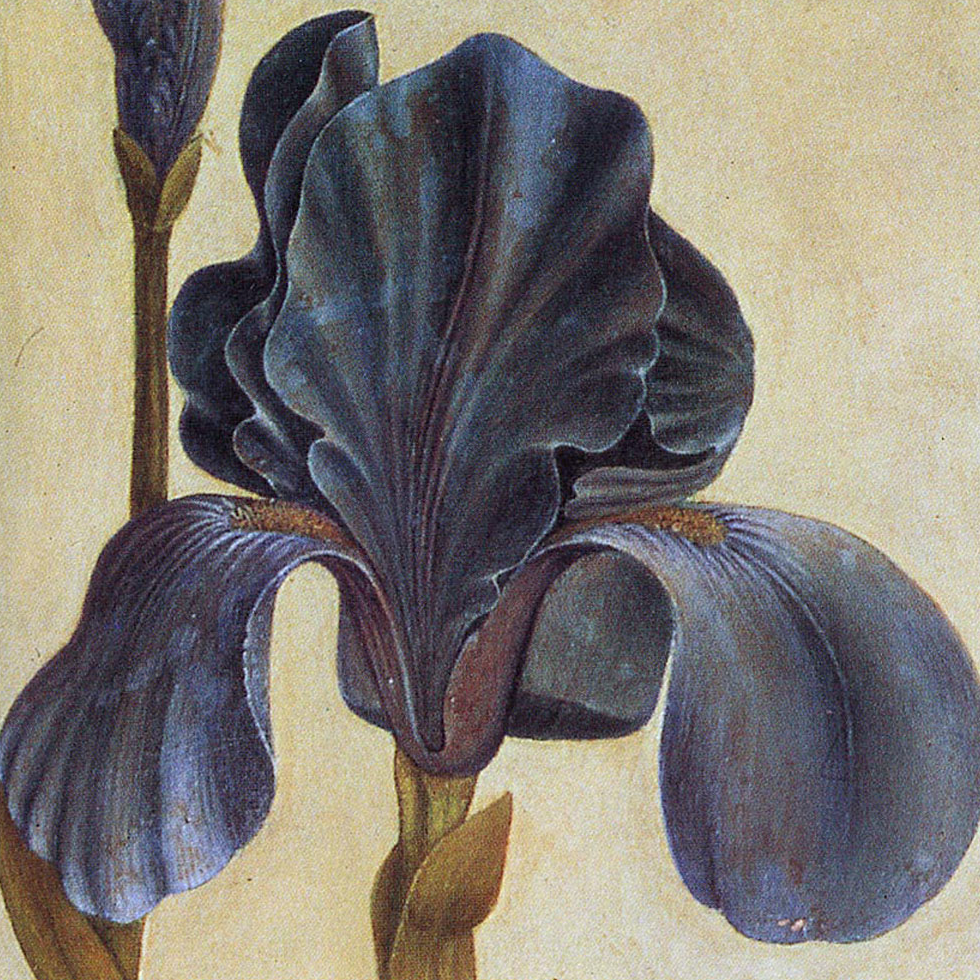
\includegraphics[scale = 0.75]{titlepage.png}\\[0.5cm]

		\textsc{\Huge\theorganization}\\
		\rule{\linewidth}{0.2 mm}\\[0.3 cm]
			{\huge\bfseries\thetitle\thesubtitle}\\
		\rule{\linewidth}{0.2 mm}\\[1 cm]

		\vfill

		\Large{\textbf{\theauthor}}\\[0.1cm]
		\large{\therepository}\\[0.5 cm]
		{\large \thedate}\\[1.5 cm]
	\end{center}

	{\doclicenseThis}
\end{titlepage}

\tableofcontents

% Document files

\chapter{Getting to know Aqademia}

\section{A \hologo{XeTeX} template for printable academic documents}

This is a custom \hologo{XeTeX} template designed for note taking and posterior printing (hence the serif font).
It's a redesign of \href{https://github.com/advy99}{advy99}'s template, which is a heavy redesign of one \href{https://github.com/Dunspa}{Dunspa} provided us with.
We regretably can't find the primary source anywhere, sorry about that.
The listings style was inspired by \href{https://github.com/Wandmalfarbe}{Wandmalfarbe}'s Eisvogel.

The placeholder image \code{src/titlepage.png} is \textit{Troiana Iris} by Albrecht Dürer.

A demo is avaliable at the \href{https://github.com/Groctel/aqademia/releases}{releases} page.

\section{Document properties}

\subsection{Physical properties}

This document is designed to be printed in European A4 paper and to fit as much text as possible in a single page without becoming too crowded (check the margins in \code{marginsrb}).
It uses \code{fancy} style headers and footers and coloured hyperlinks.

\subsection{Arguments}

This template provides some arguments to customize your document:

\begin{center}
\begin{tabular}{l l l l}
\textbf{Argument}   & \textbf{Type} & \textbf{Default}             & \textbf{Description}                                          \\
\midrule
\midrule
\code{license}      & Bool          & \code{false}                 & Whether to display the licence at the title page.             \\
\code{subtitle}     & Bool          & \code{false}                 & Whether to display the subtitle at the title page.            \\
\code{toc}          & Bool          & \code{false}                 & Whether to display the table of contents after the titlepage. \\
\code{achapter}     & String        & \code{Appendix}              & Chapter text (appendices only).                               \\
\code{author}       & String        &                              & Author of the document.                                       \\
\code{chapter}      & String        & \code{Part}                  & Chapter text.                                                 \\
\code{date}         & String        & \code{\textbackslash{}today} & Date of the last version of the document.                     \\
\code{graphics}     & String        & \code{img/}                  & Graphics directory.                                           \\
\code{language}     & String        & \code{english}               & Language provided to \code{babel}                             \\
\code{lmodifier}    & String        & \code{by-nc-sa}              & Modifier argumento for \code{doclicense}.                     \\
\code{ltitle}       & String        & \code{CC}                    & Title argument of \code{doclicense}.                          \\
\code{lversion}     & String        & \code{4.0}                   & Version argument for \code{doclicense}.                       \\
\code{organization} & String        &                              & Organisation or other supertitle.                             \\
\code{section}      & String        & \code{Session}               & Section text.                                                 \\
\code{tab}          & String        & \code{3}                     & Size of tabs in listings.                                     \\
\code{title}        & String        &                              & Title of the document.                                        \\
\code{repository}   & String        &                              & Link to the document's repository.                            \\
\code{subtitle}     & String        &                              & Subtitle of the document (titlepage only).                    \\
\end{tabular}
\end{center}


\pagebreak
\section{Dependencies}

The font used in listings is \code{Libertine Mono}\footnote{It is scaled down in inline code sections}.
The document is designed to be built with \hologo{XeTeX}.



\section{Building}

\begin{lstlisting}[language=Bash]
cd src
xelatex aqademia.tex
\end{lstlisting}


% Appendices formatting and files

\setcounter{chapter}{0}
\renewcommand{\thesection}{\MakeUppercase{\alph{chapter}}.\arabic{subsection}}
\titleformat{\chapter}[block]{\normalfont\bfseries\Huge}{Appendix\ \MakeUppercase{\alph{chapter}}:\ }{0pt}{}[]
\titleformat{\section}[block]{\normalfont\bfseries\Large}{\S\ \thesection:\ }{0pt}{}[]
\titleformat{\subsection}[block]{\normalfont\bfseries\large}{\thesubsection:\ }{0pt}{}[]

\chapter{About appendices}

\section{Differences over sessions}

While the chapter is declared outside the \code{input} files in the sessions, it is declared as the appendices header.
The \code{section} command is substituted by the \code{subsection} command previously used, so that the style is conserved without losing a sectioning level.

\subsection{Subsections}

The \code{subsection} level is also substituted by \code{subsubsection}.

\section{Numbering}

Appendices are referred to as a letter, starting from letter \code{A}.




\end{document}
